\documentclass{standalone}
\usepackage{tikz}
\usetikzlibrary{decorations.pathreplacing}

\begin{document}

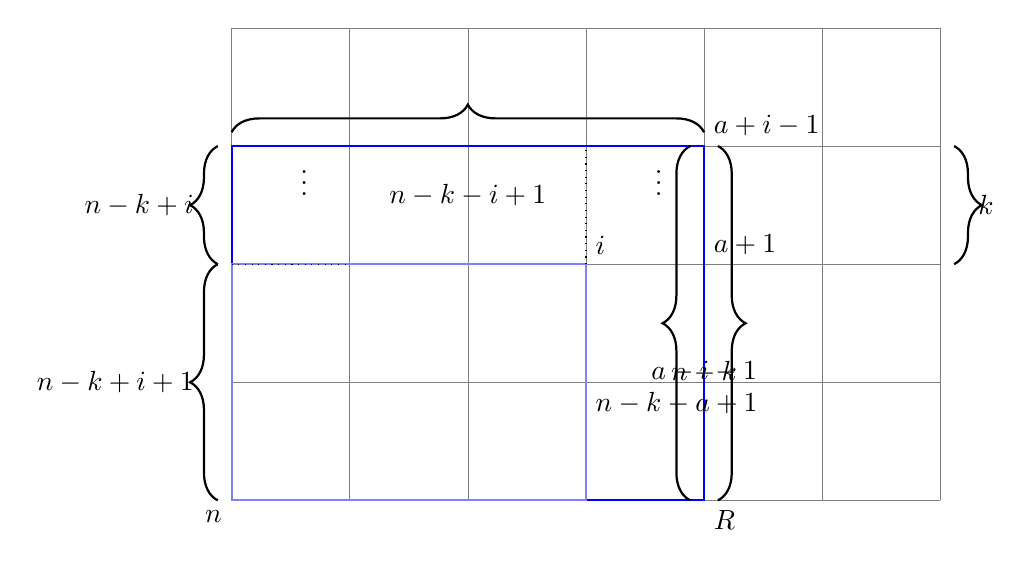
\begin{tikzpicture}[scale=1.5]
    % Draw the grid
    \draw[help lines] (0,0) grid (6,4);
    
    % Draw the main rectangle R
    \draw[thick, blue] (0,3) -- (4,3) -- (4,0) -- (0,0) -- cycle;
    
    % Marking the top-left corner of the main rectangle r
    \node at (4,3) [above right] {$a+i-1$};
    
    % Draw the smaller rectangle r
    \draw[thick, blue!50] (0,2) -- (3,2) -- (3,0) -- (0,0) -- cycle;
    
    % Marking the top-left corner of the smaller rectangle r
    \node at (3,2) [above right] {$i$};
    
    % Marking the top-right corner of the main rectangle r
    \node at (4,2) [above right] {$a+1$};
    
    % Marking the bottom-left corner of the main rectangle r
    \node at (0,0) [below left] {$n$};
    
    % Marking the bottom-right corner of the main rectangle r
    \node at (4,0) [below right] {$R$};
    
    % Labeling the vertical steps
    \draw[decorate, decoration={brace, amplitude=10pt, raise=5pt}, thick] (0,0) -- node[left=10pt] {$n-k+i+1$} (0,2);
    \draw[decorate, decoration={brace, amplitude=10pt, raise=5pt}, thick] (0,2) -- node[left=10pt] {$n-k+i$} (0,3);
    
    % Labeling the horizontal steps
    \draw[decorate, decoration={brace, amplitude=10pt, raise=5pt}, thick] (0,3) -- node[below=10pt] {$n-k-i+1$} (4,3);
    \draw[decorate, decoration={brace, amplitude=10pt, raise=5pt}, thick] (4,3) -- node[below=10pt] {$a-i-1$} (4,0);
    
    % Labeling the side length k
    \draw[decorate, decoration={brace, mirror, amplitude=10pt, raise=5pt}, thick] (6,2) -- node[right=10pt] {$k$} (6,3);
    
    % Marking the vertical and horizontal steps inside the main rectangle
    \draw[dotted] (3,2) -- (3,3);
    \node at (3.5, 2.5) [above right] {$\vdots$};
    
    \draw[dotted] (0,2) -- (1,2);
    \node at (0.5, 2.5) [above right] {$\vdots$};
    
    \node at (3,1) [below right] {$n-k-a+1$};
    
    \draw[decorate, decoration={brace, amplitude=10pt, raise=5pt}, thick] (4,0) -- node[below=10pt] {$n-k$} (4,3);
\end{tikzpicture}

\end{document}